\documentclass[tikz, border=7pt]{standalone}

\usepackage[T1]{fontenc}
\usepackage[english]{babel}
\usepackage{fourier}

\usepackage{xcolor}
\definecolor{wheat}{RGB}{245,222,179}

\usepackage{standalone}

\usepackage{tikz}
\usetikzlibrary{shapes, arrows, shadows, calc}

\usepackage{amsmath}

\tikzstyle{data}=[
  draw,
  font=\Large,
  align=center,
  minimum height=2.5em, 
  drop shadow, 
  rounded corners
]

\begin{document}
	\pgfdeclarelayer{background}
    \pgfdeclarelayer{foreground}
    \pgfsetlayers{background,main,foreground}
    
    \begin{tikzpicture}
    	\node (model) at (0,0) {\includestandalone[mode=buildnew, width=4cm]{building_model}};
        \path (model.east) + (15,0) node[data, fill={rgb,255:red,56;green,88;blue,140}, text=wheat] (geometric_features) {$v_{geom} = \begin{bmatrix}
        v_1\\v_2\\ \vdots \\ v_g
        \end{bmatrix}$};
        
        \path (model.south east) + (4, -4) node (dsm) {\fbox{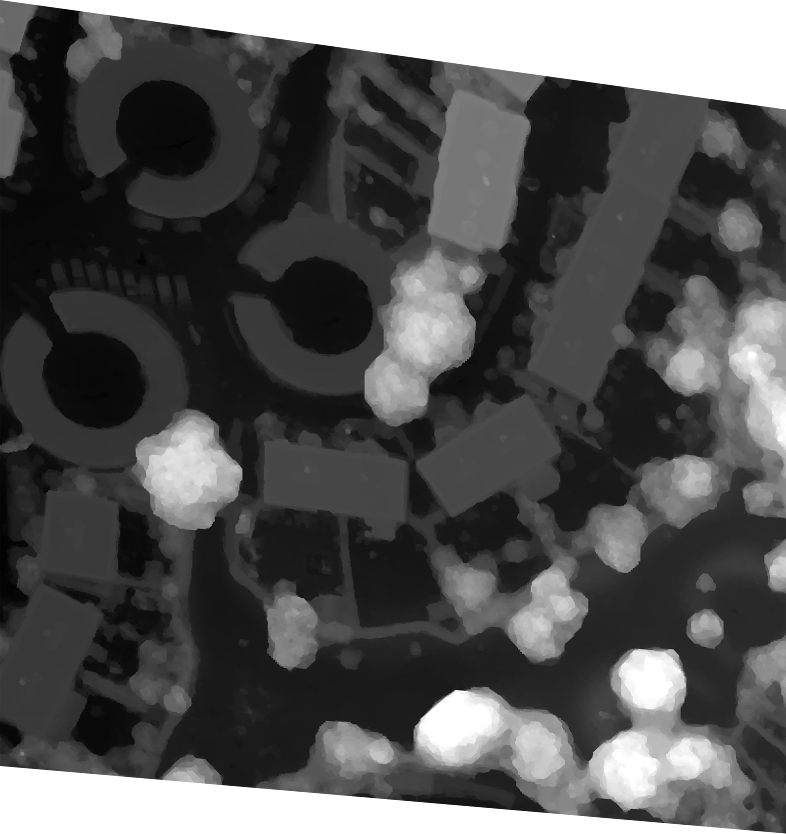
\includegraphics[width=4cm]{images/dsm_elanc}}};
        \path (dsm.north east) + (3, 1) node (simulated_dsm) {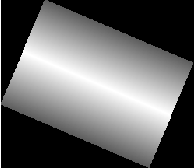
\includegraphics[width=2cm]{images/simulated_dsm}};
        \path (simulated_dsm.south |-  dsm) node (extrac_dsm) {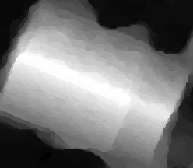
\includegraphics[width=2cm]{images/dsm}};
        \path (geometric_features |- dsm) node[data, fill={rgb,255:red,56;green,88;blue,140}, text=wheat] (altimetric_features) {$v_{alti} = \begin{bmatrix}
        v_1\\v_2\\ \vdots \\ v_a
        \end{bmatrix}$};
        
        \path (dsm.south) + (0, -7) node (orthoimage) {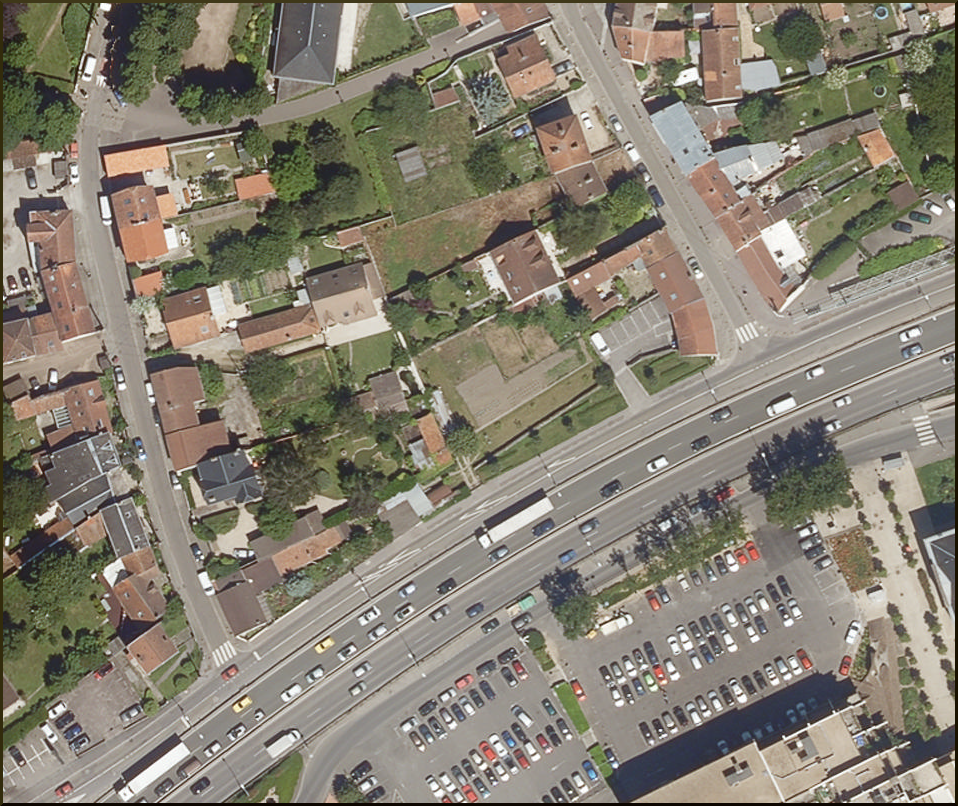
\includegraphics[width=4cm]{images/ortho_elanc}};
        \path (orthoimage.north east) + (3, 1) node (projection) {\includestandalone[mode=buildnew, width=2cm]{model_projection}};
        \path (simulated_dsm |- orthoimage) node (extrac_ortho) {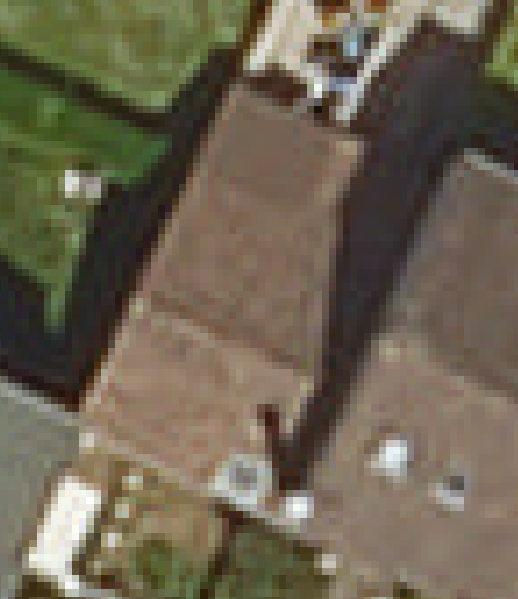
\includegraphics[width=2cm]{images/orthoimage}};
        \path (geometric_features |- orthoimage.east) node[data, fill={rgb,255:red,56;green,88;blue,140}, text=wheat] (radiometric_features) {$v_{radio} = \begin{bmatrix}
        v_1\\v_2\\ \vdots \\ v_r
        \end{bmatrix}$};
        
        \path (altimetric_features.east) + (6,0) node[data, fill={rgb,255:red,56;green,88;blue,140}, text=wheat] (features) {$feats = \begin{bmatrix}
        v_1\\v_2\\ \vdots\\ \vdots \\ v_{g+a+r}
        \end{bmatrix}$};
        \path (features) + (6,0) node[data, fill={rgb,255:red,69;green,50;blue,126}, text=white, text width=2cm] (errors) {\textsc{Error\\ list}};
        
	\begin{pgfonlayer}{background}
            \path (model.west |- simulated_dsm.north)+(-.25,.25) node (opta) {};
            \path (radiometric_features.east |- orthoimage.south)+(1,-0.25) node (optb) {};

            \path[fill=green!20, fill opacity=.5, rounded corners, draw=black!50, dashed]
                (opta) rectangle (optb);
            \path (opta.east |- optb.north)+(1,.5) node  {\Large Optional};
        \end{pgfonlayer}        
    \end{tikzpicture}
\end{document}